\section{Visualization of Network and Tree Data}
\label{sub:lr-network}

\subsection{Node-Link Diagrams}
The most common visual encoding for network and tree data is \emph{node-link diagrams}, where nodes are represented as point marks and links connecting these nodes are represented as \emph{connection} marks. We further discuss layouts using this representation for network data with different constraints of graph structure: rooted tree, directed graph and general graph.

\subsubsection{Tree Layout}
A classic algorithm by Reingold and Tilford~\cite{Reingold1981} produces a tidy tree layout satisfying the following aesthetic rules:
\begin{enumerate}
	\item Nodes at the same level of the tree should lie along a straight line, and the straight lines defining the levels should be parallel.
	\item A left son should be positioned to the left of its father, and a right son should be positioned to the right of its father.
	\item A father should be centered over its sons.
\end{enumerate} 

Even though the layout produced by Reingold and Tilford's algorithm is tidy, it still leaves plenty of void space at the root side of the tree as shown in \autoref{fig:lr-tree-tidy}. Marriott and Sbarski~\cite{Marriott2007} relax the rule that a parent must be placed at the center of its children by slightly shifting branches of nodes to produce a narrower tree. In practice, nodes have their sizes rather than just single points, and their heights can also be different. Van der Ploeg~\cite{VanderPloeg2014} relaxes the layering requirement to produce a shorter tree as shown in \autoref{fig:lr-tree-tidy-non-layer}.

\begin{figure}[!htb]
\centering
\subcaptionbox{Reingold -- Tilford algorithm. \is{Nguyen2002}\label{fig:lr-tree-tidy}}{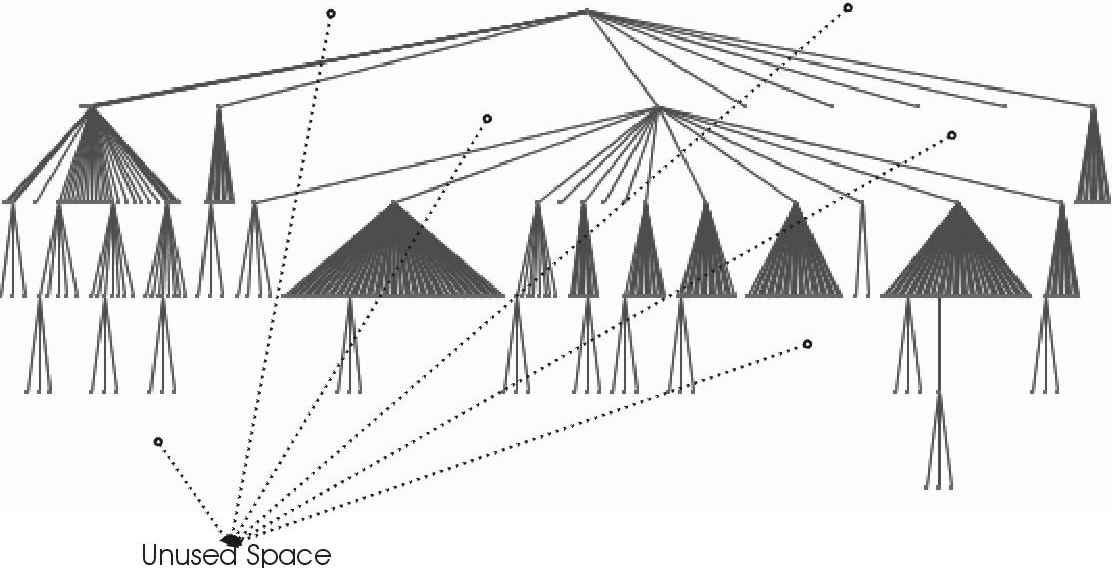
\includegraphics[height=.318\columnwidth]{tree-tidy}}
\hfill
\subcaptionbox{Relaxed layering for shorter layout. \is{VanderPloeg2014}\label{fig:lr-tree-tidy-non-layer}}{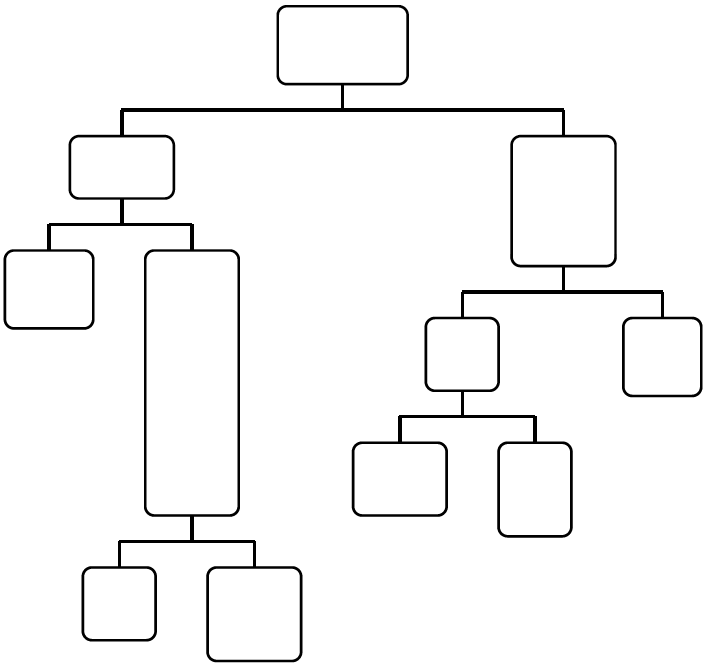
\includegraphics[height=.318\columnwidth]{tree-tidy-non-layer}}
\caption{Tree layouts.}
\end{figure}

Conventionally, tree layouts are rectilinear with children branching from the parent node either from left to right or top to bottom. However, the children nodes can also be arranged radially, along a circular arc of their parent. The depth of a circular tree is encoded as distance away from the center of the circle. Reingold -- Tilford algorithm can be modified to show a radial tree. The radial version could be a bit more compact than the linear one and because the outer layer is longer than the inner ones, it has more space to show its nodes. However, it could be easier to see the hierarchical structure with the linear structure because of its familiarity. \autoref{fig:lr-tree} shows the class hierarchy of the \emph{Flare} visualization toolkit~\cite{Heer2009b} using both a conventional tree and a radial tree. The toolkit consists of 10 top-level classes, which determine the color of nodes in these figures.

\begin{figure}[!htb]
\centering
\subcaptionbox{Conventional tree, growing direction as left to right. \label{fig:lr-tree-rect}}[.3\columnwidth]{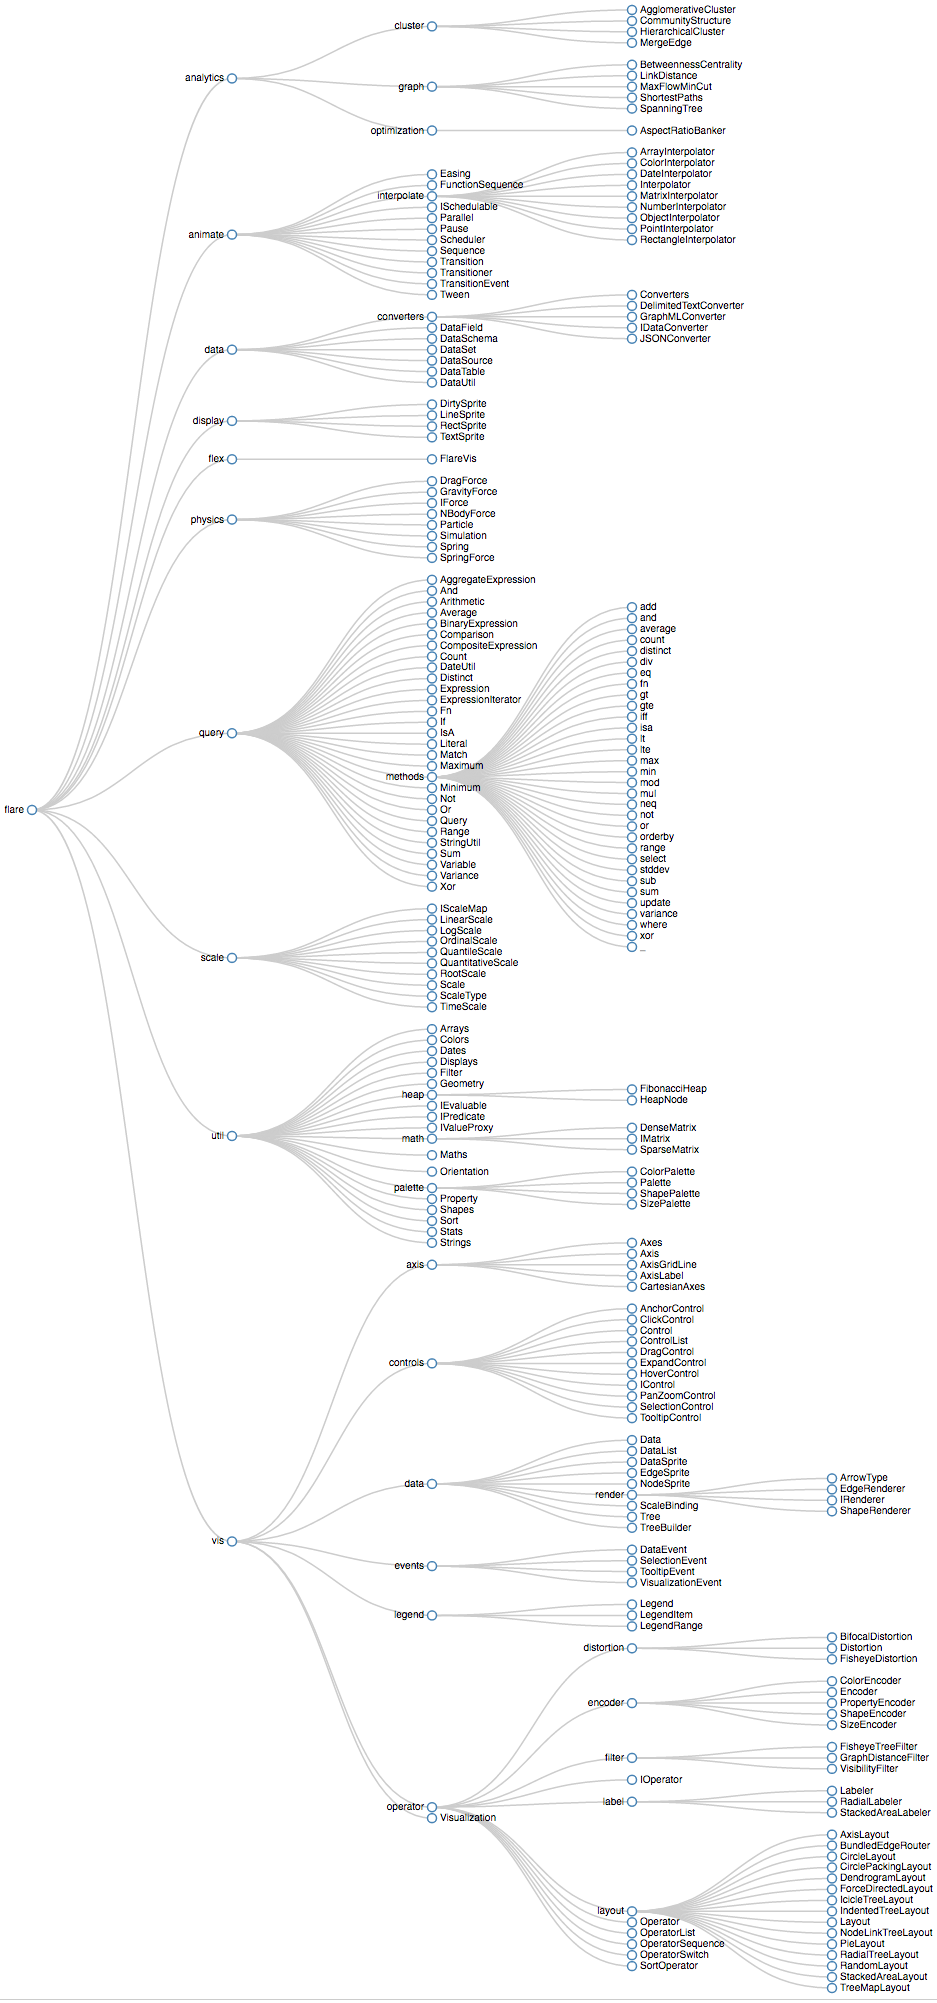
\includegraphics[height=.6\columnwidth]{tree-rect}}
\hfill
\subcaptionbox{Radial tree. Depth is encoded as distance away from the center. \label{fig:lr-tree-radial}}[.65\columnwidth]{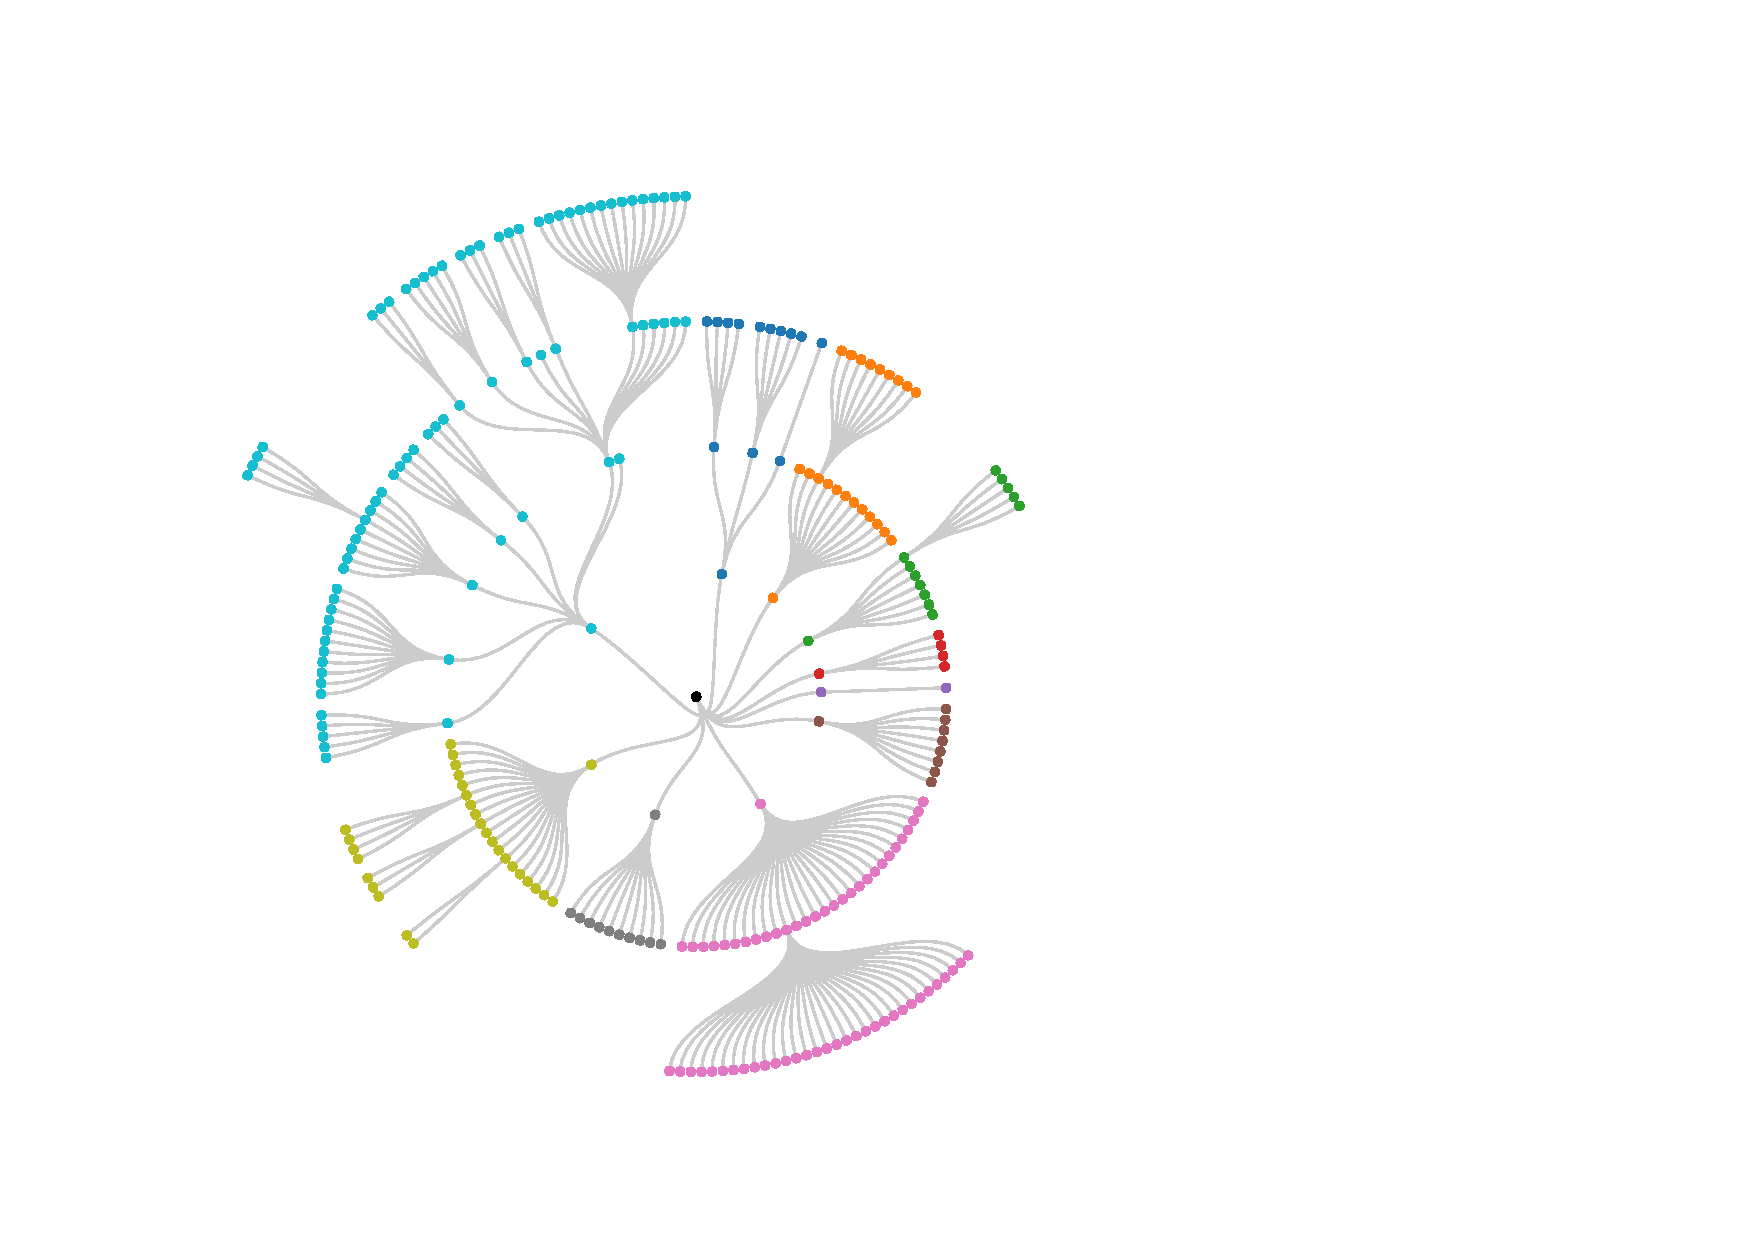
\includegraphics[height=.6\columnwidth]{tree-radial}}
\caption[Tree layouts with different orientations]{Tree layouts with different orientations. Data is the class hierarchy of the Flare visualization toolkit~\cite{Heer2009b} with color representing the top-level classes.}
\label{fig:lr-tree}
\end{figure}
  
\subsubsection{Directed Graphs -- Hierarchical Graph Layout}	
The most popular method of drawing directed graphs is the Sugiyama method~\cite{Sugiyama1981}, which separates nodes into layers to show the hierarchy effectively (\autoref{fig:lr-layered-graph}). The method consists of four steps.

\begin{figure}[!htb]
	\centering
	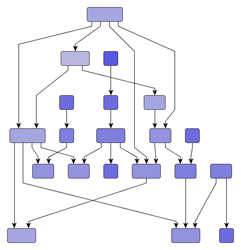
\includegraphics[width=.3\columnwidth]{layered-graph}
	\caption[A layered graph]{A layered graph. Nodes are assigned to horizontal layers. Within each layer, nodes are ordered to minimize edge crossings and assigned x-coordinate to make edges as straight as possible. \textrm{\emph{Image source: yWorks.}}}
	\label{fig:lr-layered-graph}
\end{figure}

\begin{enumerate}
	\item \emph{Cycle removal}. If the input graph contains directed cycles, the directions of some edges are temporarily reversed to make the graph acyclic.
	\item \emph{Layer assignment}. Nodes are assigned to horizontal layers, which determines their y-coordinates.
	\item \emph{Vertex ordering}. Within each layer, the nodes are ordered to minimize edge crossings between adjacent layers.
	\item \emph{Horizontal coordinate assignment}. The x-coordinate of each node is determined, typically aiming to make edges straight.
\end{enumerate}

\subsubsection{General Graph -- Force-Directed Layout}
Force-directed layout~\cite{Eades1984} is a popular method to visualize general graphs using node-link metaphor. It positions nodes based on a simulation of physical forces: \emph{spring-like attractive} forces attract nodes, and \emph{repulsive} forces like those of electrically charged particles push them away from each other. The layout usually starts with a random arrangement of nodes and then iteratively refines their locations according to the behavior of the simulation. The simulation stops when it reaches a stable state or a maximum number of iterations. \autoref{fig:lr-force-directed-idea} illustrates the idea of physical simulation, and \autoref{fig:lr-force-directed-example} shows an example with color indicating node type.

\begin{figure}[!htb]
\centering
\subcaptionbox{A physical simulation. \label{fig:lr-force-directed-idea}}{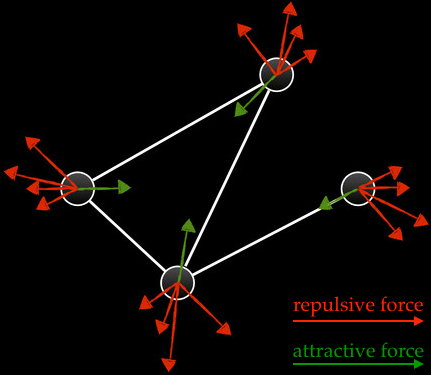
\includegraphics[height=.25\columnwidth]{force-directed-idea}}
\hspace{1cm}
\subcaptionbox{An example with color showing node type. \label{fig:lr-force-directed-example}}{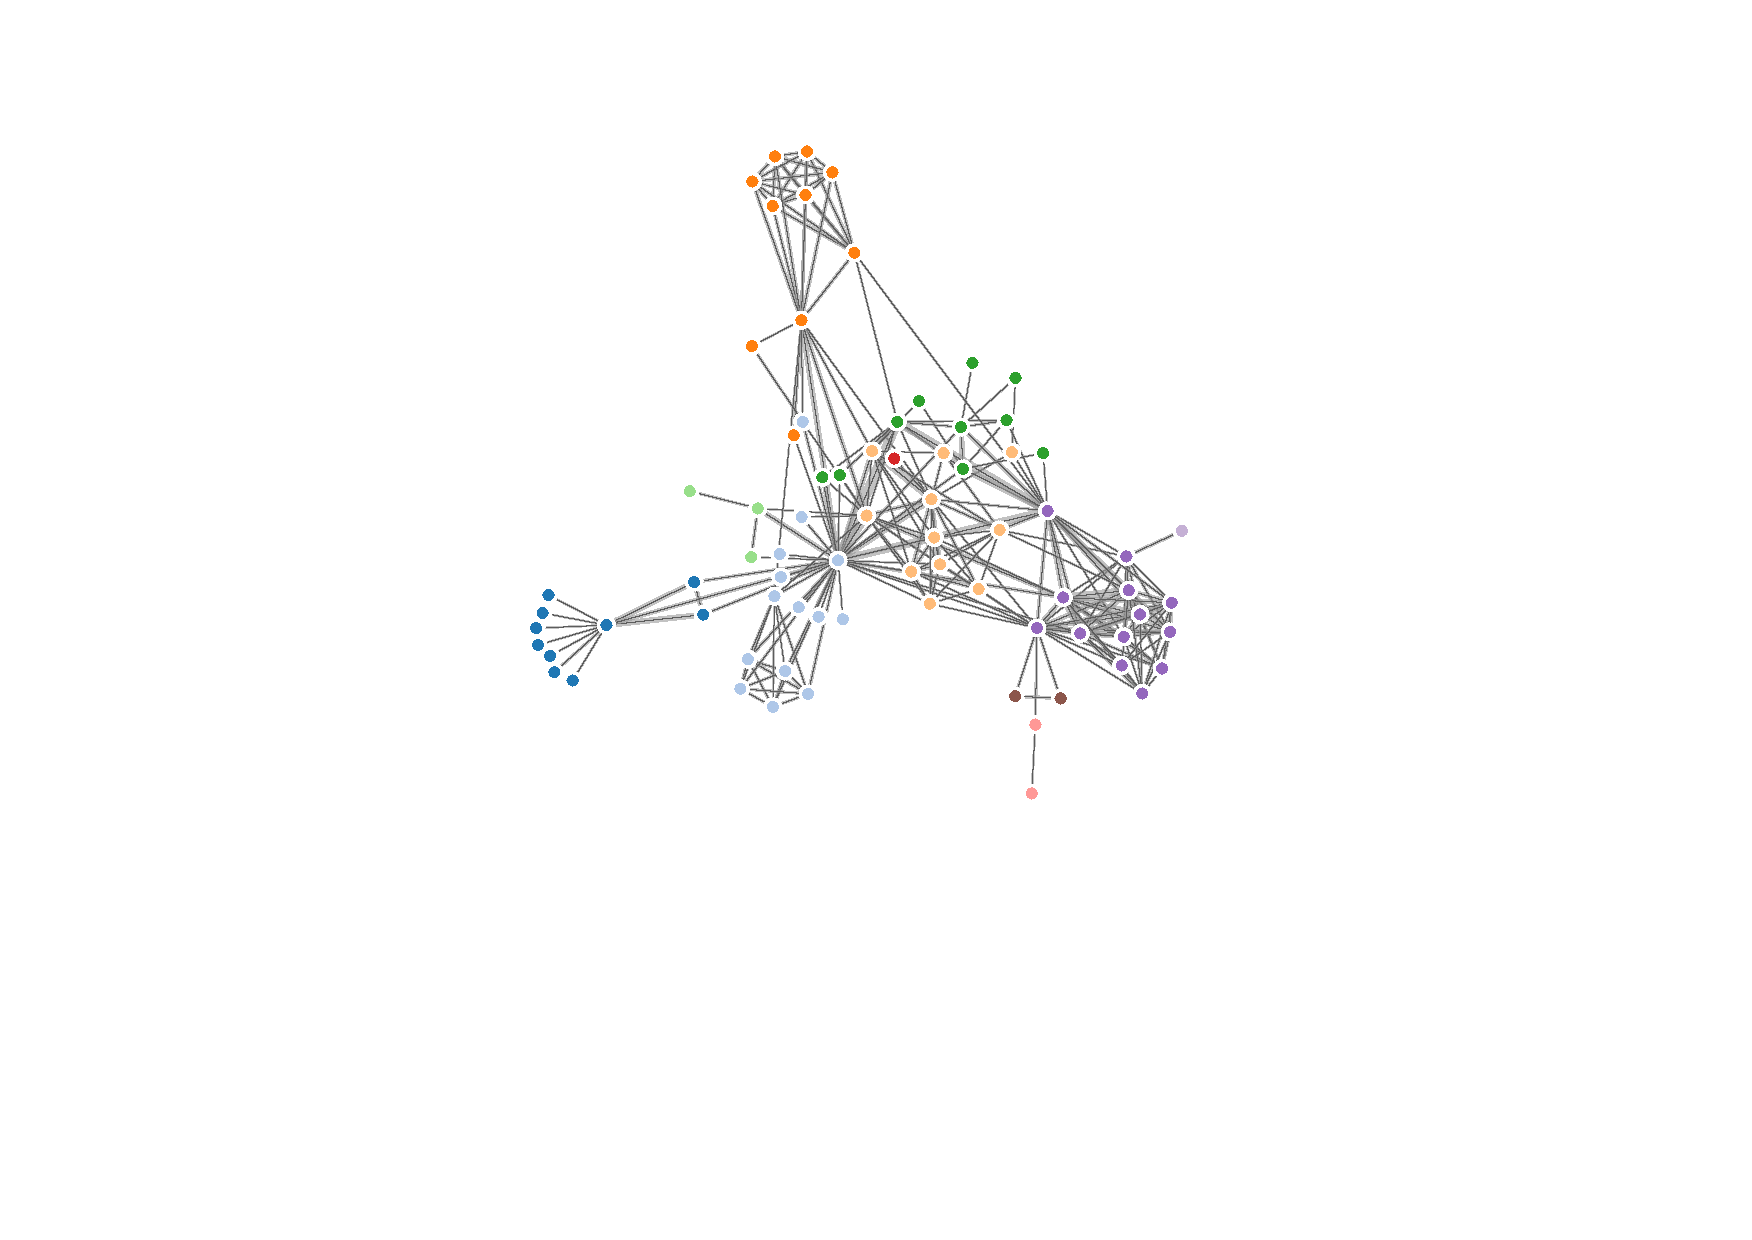
\includegraphics[height=.5\columnwidth]{force-directed-example}}
\caption{Force-directed layout.}
\end{figure}

Force-directed layout is aesthetically pleasing, aiming to produce uniform edge length, symmetry and even node distribution~\cite{Fruchterman1991}. However, its major weakness is scalability, in terms of both the visual complexity and the running time~\cite{Munzner2014}. The layout quickly degenerates into a hairball of visual clutter with even a few hundred nodes. Another limitation is its nondeterministic output: the layout looks different each time it runs, breaking user mental model.

\subsection{Matrix Views}
A network can be represented by an adjacency matrix. Each row and column of the matrix corresponds to a node, and a cell indicates whether the pair of corresponding nodes is connected in the network. Additional information about edges are often encoded to the visual representation of cells using color, shape and size. Matrix views can also show weighted networks, where each link associates with a quantitative value attribute, by encoding cells with an ordered visual channel such as color luminance or size. \autoref{fig:lr-matrix} shows examples of matrix views, compared with node-link diagrams of the same datasets.

\begin{figure}[!htb]
\centering
\subcaptionbox{Comparison with a small network. \label{fig:lr-matrix-1}}{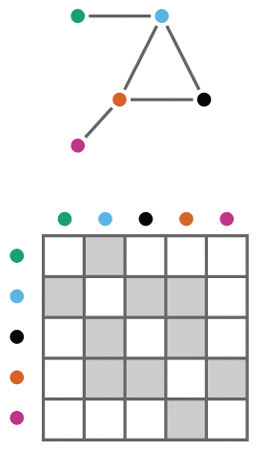
\includegraphics[height=.39\columnwidth]{matrix-1}}
\hfill
\subcaptionbox{Matrix view of larger network. \label{fig:lr-matrix-2}}{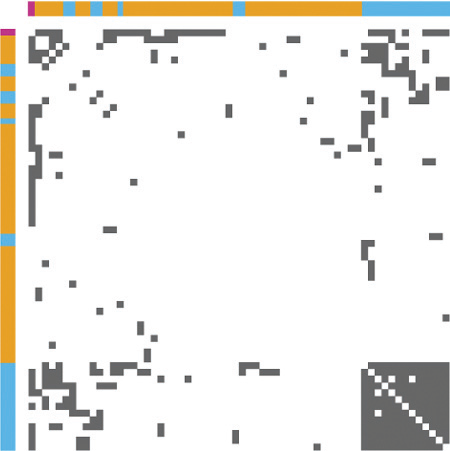
\includegraphics[height=.39\columnwidth]{matrix-2}}
\hfill
\subcaptionbox{Force-directed layout of larger network. \label{fig:lr-matrix-3}}{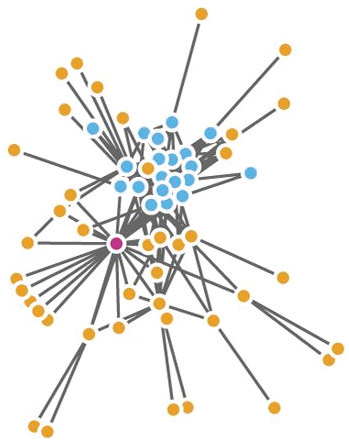
\includegraphics[height=.39\columnwidth]{matrix-3}}
\caption[Comparison of node-link diagrams and matrix views]{Comparison of node-link diagrams and matrix views. Gray cells indicate edge connectivity. \is{Munzner2014}}
\label{fig:lr-matrix}
\end{figure}

A major strength of matrix views is the scalability. It can easily show a network with thousands of nodes and millions of edges without suffering from the cluttering issue as in node-link diagrams. Matrix views are also stable: adding a new node or edge will only cause a small visual change. Whereas, adding a new item in a force-directed view may lead to a major change~\cite{Munzner2014}. Nodes, as columns and rows in a matrix view, can be reordered, allowing users to reveal outliers, clusters, and patterns of the network~\cite{Henry2007}.

A major weakness of matrix views is their difficulty in exploring the topological structure of the network, such as path tracing. This because they show links in a more indirect way than the direct connections of node-link diagrams -- a trade-off for their strength in avoiding clutter. Another weakness of matrix views is unfamiliarity: users easily interpret small node-link diagrams but require training to understand matrix views~\cite{Munzner2014}. A study shows that for many low-level abstract network tasks, node-link diagrams are best for small networks, whereas matrix views are best for large networks~\cite{Ghoniem2005}.

\subsection{Space-Filling Techniques}
Space-filling techniques can only be applied to tree data and uses \emph{containment} marks to represent hierarchical relationship, placing child nodes within their parent node. Treemap~\cite{Shneiderman1992} represents a node as a rectangle, which is recursively subdivided into smaller rectangles, each representing a child of the node. The rectangle size is proportional to a quantitative attribute of its node. The original motivation of treemap is to analyze the utilization of storage space on a hard disk. Each leaf node represents a computer file, and the node size encodes the file size. The size of a parent node simply maps to the containing folder size. Color is also commonly used to encode additional information to nodes such as file type. \autoref{fig:lr-treemap} shows such an example of treemap.

\begin{figure}[!htb]
	\centering
	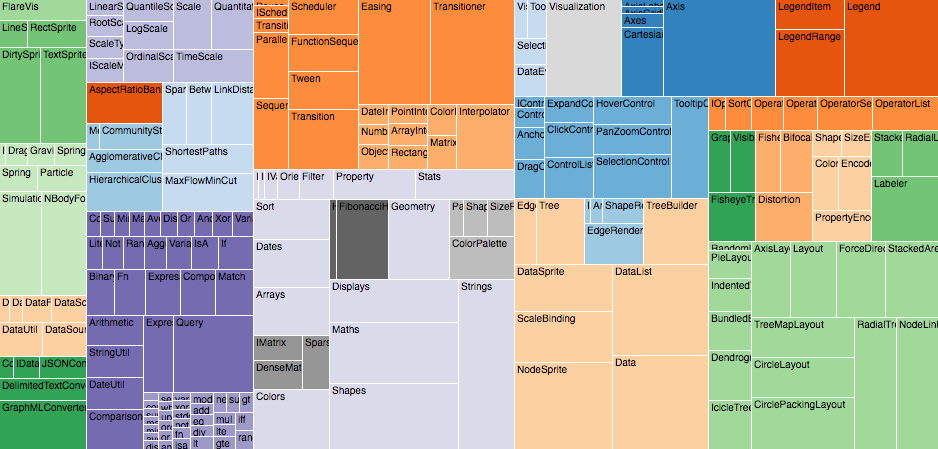
\includegraphics[width=.7\columnwidth]{treemap}
	\caption[Treemap]{Treemap showing the class hierarchy of the Flare visualization toolkit~\cite{Heer2009b}. Area represents class sizes and color represents the top-level classes.}
	\label{fig:lr-treemap}
\end{figure}

Treemap is very effective when size is the most important feature to be displayed. It easily spots outliers of very large attribute values such as large files. However, containment is not as effective as connection in node-link diagrams for tasks focused on topological structure. It is difficult to identify the path of a given node, thus suitable for hierarchies with just a few levels. Borders of nodes or shading can be used to depict the tree structure more strongly~\cite{Wijk1999}.

Alternatively, other space-filling techniques have been proposed to represent the hierarchical structure more effectively. \autoref{fig:lr-other-space-filling} shows three techniques that will be discussed next using the same dataset as in \autoref{fig:lr-treemap} for treemap. 

\begin{figure}[!htb]
	\centering
	\subcaptionbox{Circle packing. Circle containment indicates parent-child relationship. Circle size represents a quantitative attribute.  \label{fig:lr-circle-pack}}[.47\columnwidth]{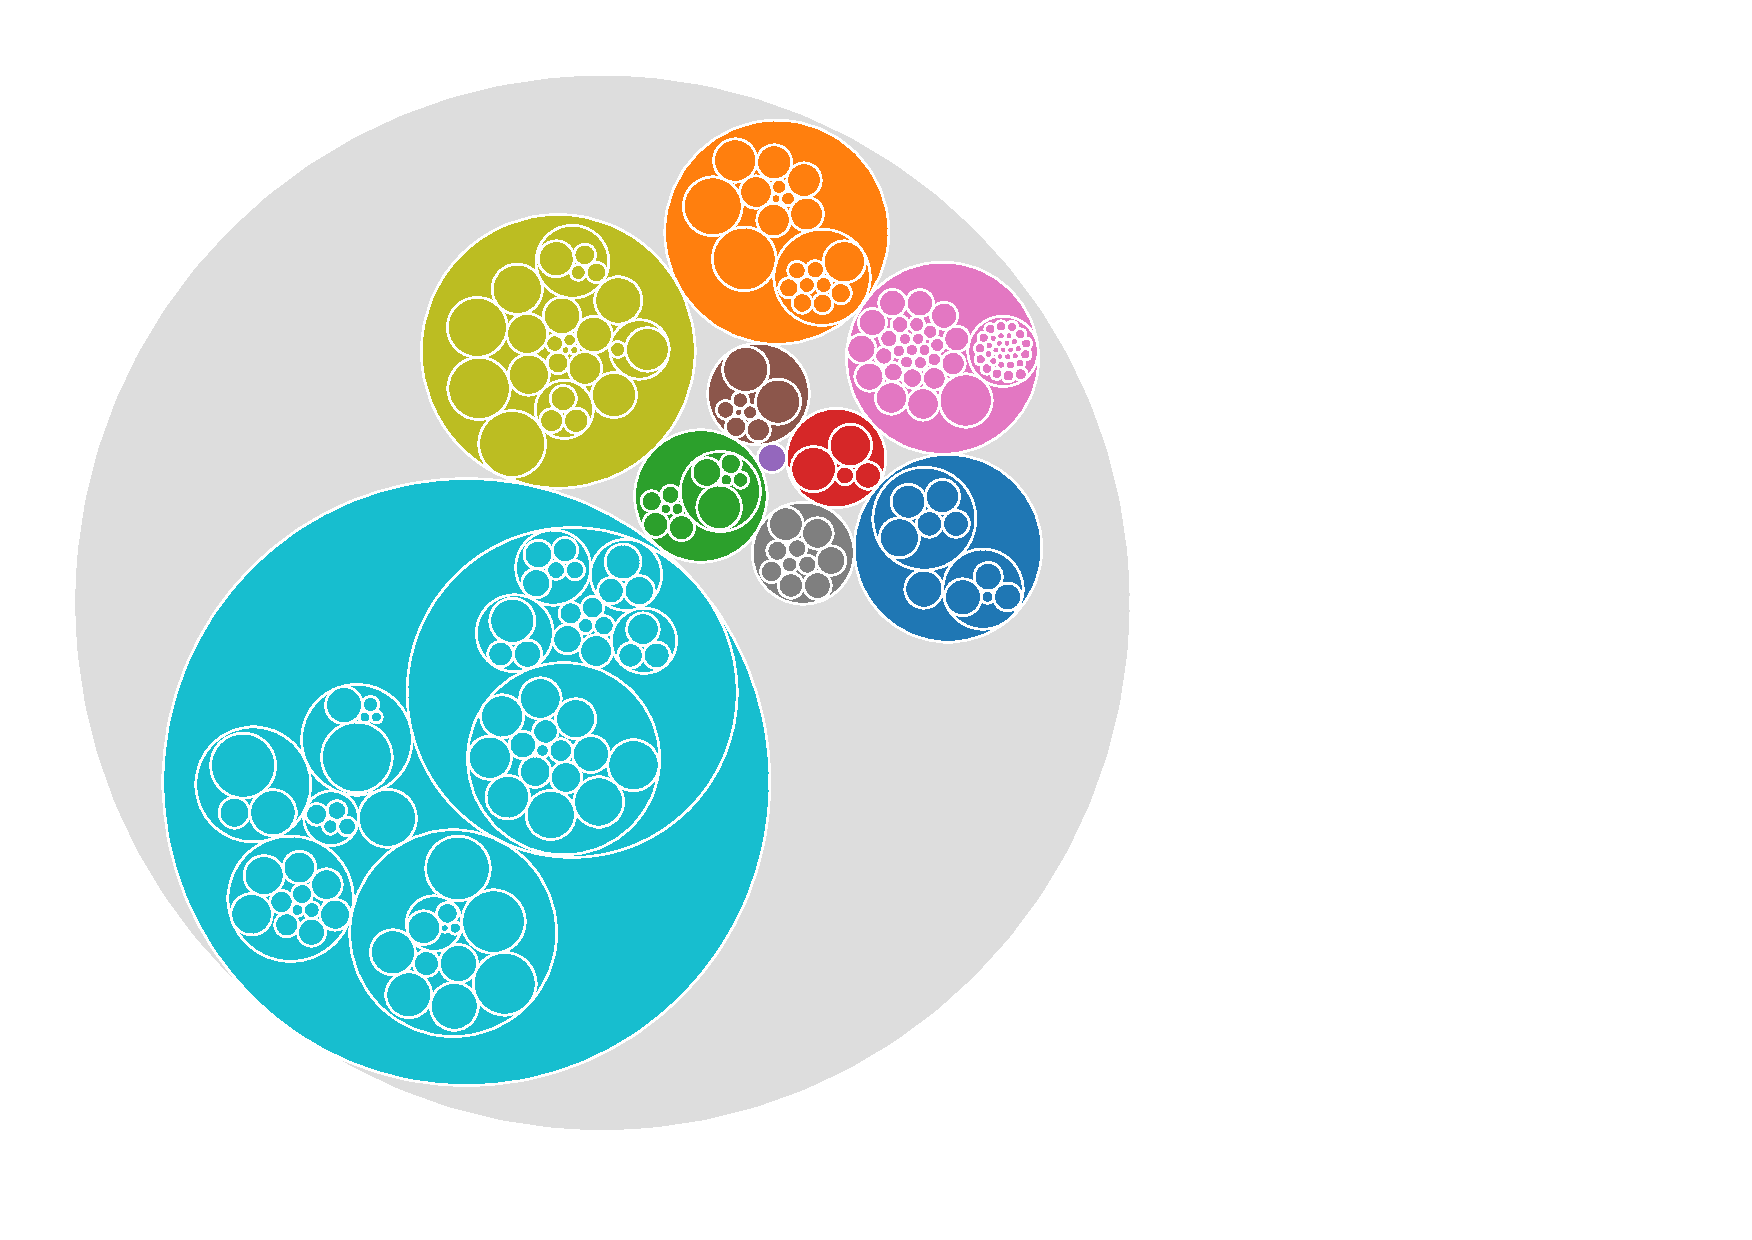
\includegraphics[height=.35\columnwidth]{circle-pack}}
	\hfill
	\subcaptionbox{Sunburst. A curved segment is the parent of its next outer segments. Segment angle represents a quantitative attribute.  \label{fig:lr-sunburst}}[.47\columnwidth]{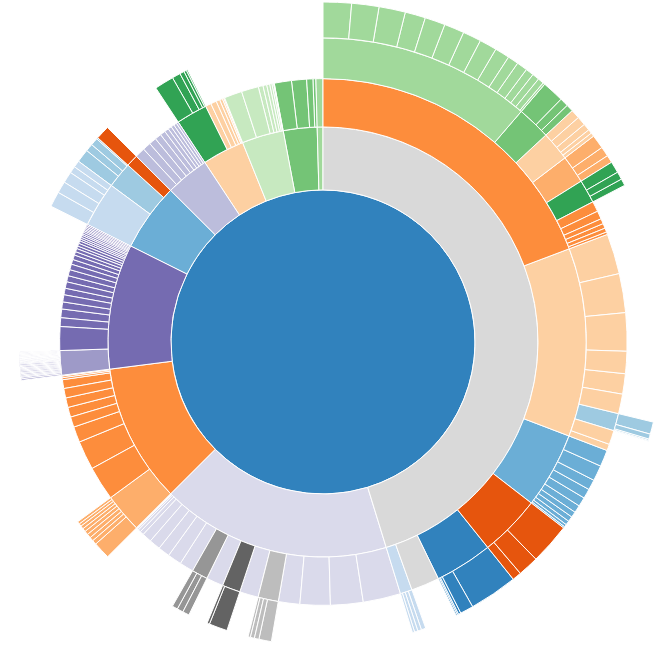
\includegraphics[height=.35\columnwidth]{sunburst}}
	
	\vspace{.5\baselineskip}
	
	\subcaptionbox{Icicle plot. A rectangle is the parent of rectangles under it. Rectangle width represents a quantitative attribute. \label{fig:lr-icile}}[\columnwidth]{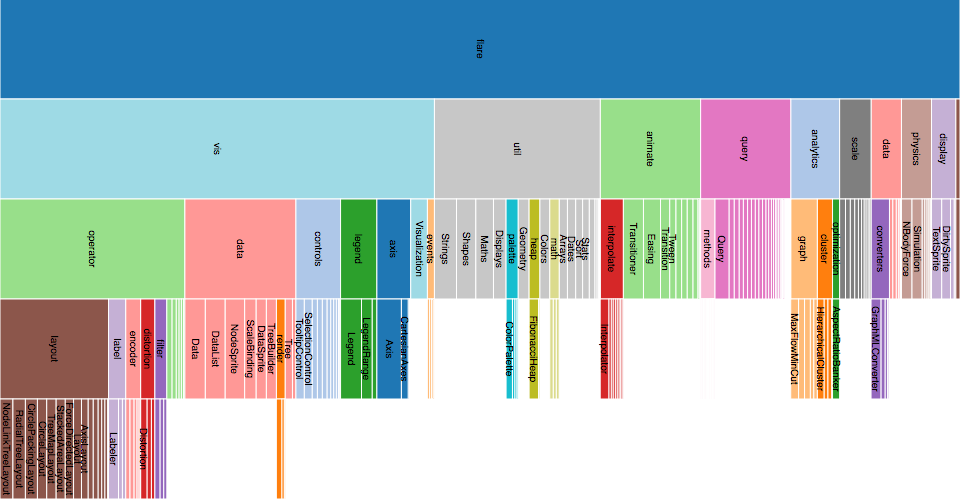
\includegraphics[width=.7\columnwidth]{icicle-plot}}
	\caption[Other space-filling techniques]{Other space-filling techniques using the same dataset as in \autoref{fig:lr-treemap}. Color also represents the top-level classes of the Flare visualization toolkit~\cite{Heer2009b}.}
	\label{fig:lr-other-space-filling}
\end{figure}

Circle packing~\cite{Wang2006} also employs containment to represent the hierarchy, but using circles to show nodes. Similar to rectangle size in treemap, the circle size also corresponds to some node value. All child nodes are packed into their parent node so that they are tangent to some of their sibling nodes. This method uses more space than treemap, but actually the additional void space helps convey the hierarchy structure more easily.

Icicle plot~\cite{Kruskal1983} does not strictly use containment; instead, it places child nodes \emph{under} their parent node. Similar to treemap, icicle plot uses rectangles to represent nodes, but they all share the same height. Therefore, node width corresponds to some attribute value. Icicle plot shows parent nodes explicitly, making it more effective in tasks related to the parents such as comparing directories by size. The direct trade-off is space for showing those parent nodes. Icicle plot shows the tree structure and supports path tracing more effectively than treemap. However, small leaf nodes are very thin and difficult to read its label or to interact with.

Sunburst~\cite{Zhang2000} is a radial version of icicle plot. Child nodes are located under their parent node in a circular layout. The root node is at the center and deeper levels are further away from it. The angle swept out by a node, or a curved segment, corresponds to its value. Color is also commonly used to represent additional information.

%circle packing: https://bl.ocks.org/mbostock/4063530
%sunburst: http://bl.ocks.org/mbostock/4348373
%treemap: https://bl.ocks.org/mbostock/4063582
%icile: https://bl.ocks.org/mbostock/1005873

\subsection{Summary}
This section reviews the most common techniques to visualize network data including node-link diagrams, matrix views and space-filling. Node-link diagrams are user-friendly and suitable for small datasets, whereas matrix views are better at large datasets. Space-filling techniques produce a compact visualization of tree data and are effective in using size to represent a quantitative attribute. \autoref{chap:sensemap} also uses network data showing pair-wise relationship between provenance data items. Even though it applies an existing tree layout, the research discussed in this section lays the foundation for making suitable design decision. To address scalability, our tree visualization includes representations for different levels of detail and interactive features such as semantic zooming and panning.